\tikzstyle{input_neuron}=[circle,draw=red!50,fill=red!10,thick,minimum size=6mm]
\tikzstyle{hidden_neuron}=[circle,draw=blue!50,fill=cyan!10,thick,minimum size=6mm]
\tikzstyle{output_neuron}=[circle,draw=green!50,fill=green!10,thick,minimum size=6mm]

\tikzstyle{input}=[circle,draw=black!50,fill=black!20,thick,minimum size=6mm]

\begin{center}
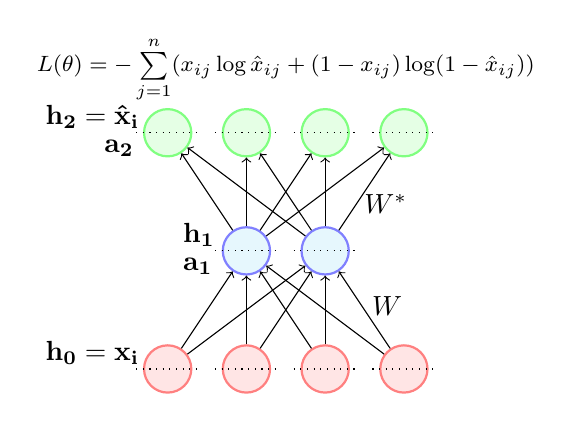
\begin{tikzpicture}


\node [input_neuron] (neuron01) at (6.5,4.5) {};
\node [input_neuron] (neuron02) at (7.5,4.5){};
\node [input_neuron] (neuron03) at (8.5,4.5) {};
\node [input_neuron] (neuron04) at (9.5,4.5) {};

\node [hidden_neuron] (neuron51) at (7.5,6) {} ;
\node [hidden_neuron] (neuron52) at (8.5,6)  {};

\node [output_neuron] (neuron11) at (6.5,7.5)  {};
\node [output_neuron] (neuron12) at (7.5,7.5)  {};
\node [output_neuron] (neuron13) at (8.5,7.5)  {};
\node [output_neuron] (neuron14) at (9.5,7.5)  {};

\node[] (lossexp) at (8,8.3)  {\footnotesize{$ \mathscr{L(\theta)} =  -\sum\limits_{j=1}^n(x_{ij}\log\hat{x}_{ij} + (1-x_{ij}) \log(1-\hat{x}_{ij})) $}};

\node[text width=1.5cm] at (5.7,4.7) {$\mathbf{h_0}=\mathbf{x_i}$};
\node[text width=0.005cm] at (6.7,6.2) {$\mathbf{h_1}$};
\node[text width=0.005cm] at (6.7,5.8) {$\mathbf{a_1}$};
\node[text width=1.5cm] at (5.7,7.7) {$\mathbf{h_2}=\mathbf{\hat{x}_i}$};
\node[text width=0.005cm] at (5.7,7.3) {$\mathbf{a_2}$};
\node[text width=0.005cm] at (9.1,5.3) {$W$};
\node[text width=0.005cm] at (9,6.6) {$W^*$};

\draw [dotted] (6.1,4.5) -- (6.9,4.5);
\draw [dotted] (7.1,4.5) -- (7.9,4.5);
\draw [dotted] (8.1,4.5) -- (8.9,4.5);
\draw [dotted] (9.1,4.5) -- (9.9,4.5);

\draw [dotted] (7.1,6) -- (7.9,6);
\draw [dotted] (8.1,6) -- (8.9,6);

\draw [dotted] (6.1,7.5) -- (6.9,7.5);
\draw [dotted] (7.1,7.5) -- (7.9,7.5);
\draw [dotted] (8.1,7.5) -- (8.9,7.5);
\draw [dotted] (9.1,7.5) -- (9.9,7.5);
\draw[->](neuron01) -- (neuron51);
\draw[->](neuron01) -- (neuron52);
\draw[->](neuron02) -- (neuron51);
\draw[->](neuron02) -- (neuron52);
\draw[->](neuron03) -- (neuron51);
\draw[->](neuron03) -- (neuron52);
\draw[->](neuron04) -- (neuron51);
\draw[->](neuron04) -- (neuron52);

\draw[->](neuron51) -- (neuron11);
\draw[->](neuron51) -- (neuron12);
\draw[->](neuron51) -- (neuron13);
\draw[->](neuron51) -- (neuron14);

\draw[->](neuron52) -- (neuron11);
\draw[->](neuron52) -- (neuron12);
\draw[->](neuron52) -- (neuron13);
\draw[->](neuron52) -- (neuron14);

\end{tikzpicture}
\end{center}
